% The design loop of spacetime engineering, drawn across both columns.
\documentclass[tikz,border=1pt]{standalone}
% Shared preamble for the standalone figures: the book's fonts, palette and
% drawing styles. Figures are drawn at their final printed size. A column is
% 3.35in (241pt) wide; a figure across both columns is 7in (505pt) wide.

\usepackage[T1]{fontenc}
\usepackage{newpxtext}
\usepackage[varbb]{newpxmath}
\usepackage[semibold,scale=0.95,lining]{sourcesanspro}
\usepackage{xcolor}
% Palette shared by the book and by the standalone figures in figures/src.
% One main hue (blue), one accent (orange), and a few roles used sparingly.

\definecolor{seblue}{HTML}{1D5B8F}    % headings, worked examples, main curves
\definecolor{seblueDark}{HTML}{123E63}
\definecolor{seorange}{HTML}{DC7A26}  % thought experiments, light and light cones
\definecolor{seteal}{HTML}{1F8577}    % checks, travellers and ships
\definecolor{sered}{HTML}{C0392B}     % negative energy, tension, violations
\definecolor{seviolet}{HTML}{5E548E}  % going deeper
\definecolor{sesand}{HTML}{8C6A3F}    % history
\definecolor{segray}{HTML}{6B7480}    % axes, guides, secondary labels
\definecolor{selight}{HTML}{D5DAE1}   % grids and faint rules

\usepackage{siunitx}
\usepackage{fontawesome5}
\usepackage{tikz}
\usetikzlibrary{arrows.meta,calc,positioning,decorations.pathreplacing,
  decorations.markings,shapes.geometric,fadings,shadings,patterns,3d,
  intersections,backgrounds}
\usepackage{pgfplots}
\pgfplotsset{compat=1.18}
\usepgfplotslibrary{fillbetween,groupplots,colormaps}

\tikzset{
  >={Latex[length=2.1mm,width=1.4mm]},
  every picture/.style={line cap=round, line join=round},
  lbl/.style={font=\sffamily\footnotesize, text=black!85},
  smalllbl/.style={font=\sffamily\scriptsize, text=black!75},
  guide/.style={segray, line width=0.4pt},
  axisline/.style={segray, line width=0.5pt, -{Latex[length=1.7mm,width=1.1mm]}},
  light/.style={seorange, line width=0.9pt},
  lightdash/.style={seorange, line width=0.9pt, dash pattern=on 3pt off 2pt},
  ship/.style={seteal, line width=1.4pt},
  cone/.style={fill=seorange!22, draw=seorange!85!black, line width=0.35pt},
}

\pgfplotsset{
  se axis/.style={
    axis lines=left,
    axis line style={segray, line width=0.5pt, -{Latex[length=1.6mm,width=1.1mm]}},
    tick style={segray, line width=0.4pt},
    major tick length=2.5pt,
    tick label style={font=\sffamily\scriptsize, text=black!75},
    label style={font=\sffamily\footnotesize, text=black!85},
    every axis plot/.append style={line width=1.1pt},
    legend style={font=\sffamily\scriptsize, draw=none, fill=none},
    scaled ticks=false,
    xticklabel={\sansnum{\tick}}, yticklabel={\sansnum{\tick}},
  },
}

% Numbers in figures are set in the sans-serif text font, with a true minus.
\sisetup{mode=text, reset-text-family=false, reset-text-series=false,
  reset-text-shape=false, drop-zero-decimal, group-minimum-digits=5}
% Tick values arrive as long decimals (1.5000000000); parse them first.
\newcommand{\sansnum}[1]{\begingroup\pgfkeys{/pgf/fpu=false}%
  \pgfmathparse{1*(#1)}\num{\pgfmathresult}\endgroup}

\begin{document}
\begin{tikzpicture}[
  tile/.style={rounded corners=5pt, fill=seblue!7, draw=seblue!35, line width=0.5pt,
    minimum width=80pt, minimum height=64pt},
  stage/.style={font=\sffamily\bfseries\small, text=seblue, text height=1.7ex, text depth=0.5ex},
  desc/.style={font=\sffamily\scriptsize, text=black!70, align=center, text width=86pt},
  flowarrow/.style={-{Latex[length=2.4mm,width=1.7mm]}, seblue!75, line width=1.1pt},
  loopback/.style={-{Latex[length=2.4mm,width=1.7mm]}, seorange!90!black, line width=1.0pt},
  badge/.style={circle, fill=seblue, text=white, font=\sffamily\bfseries\tiny,
    inner sep=0pt, minimum size=9pt},
]
\def\gap{102pt}
\foreach \i in {0,...,4} {
  \node[tile] (t\i) at (\i*\gap,0) {};
  \node[badge] at ($(t\i.north west)+(7pt,-7pt)$) {\the\numexpr\i+1\relax};
}
\foreach \i/\j in {0/1,1/2,2/3,3/4}
  \draw[flowarrow] (t\i.east) ++(3pt,0) -- ($(t\j.west)+(-3pt,0)$);

% --- 1. purpose: a trip from Earth to a star
\begin{scope}[shift={(t0.center)}]
  \shade[ball color=seblue!55] (-22pt,-12pt) circle (7pt);
  \node[star, star points=5, star point ratio=2.3, fill=seorange, minimum size=13pt,
    inner sep=0pt] at (23pt,13pt) {};
  \draw[seteal, line width=0.8pt, dash pattern=on 2.2pt off 1.6pt,
    -{Latex[length=1.8mm,width=1.4mm]}]
    (-14pt,-6pt) .. controls (-6pt,10pt) and (4pt,14pt) .. (14pt,13pt);
\end{scope}

% --- 2. geometry: a curved sheet
\begin{axis}[
  at={(t1.center)}, anchor=center, width=112pt, height=100pt,
  hide axis, view={25}{32}, clip=false,
  xmin=-2, xmax=2, ymin=-2, ymax=2, zmin=-1.3, zmax=0.3,
]
\addplot3[surf, shader=faceted, faceted color=seblue!80, line width=0.3pt,
  colormap={sheet}{color=(seblue!55) color=(seblue!8)}, point meta=z,
  z buffer=sort, samples=15, samples y=15, domain=-2:2, y domain=-2:2]
  {-1.15*exp(-(x^2+y^2)/0.8)};
\end{axis}

% --- 3. demand: negative energy at a bubble wall
\begin{scope}[shift={(t2.center)}]
  \draw[segray, line width=0.4pt] (-32pt,6pt) -- (32pt,6pt);
  \fill[sered!75, domain=-30:30, samples=90, variable=\x]
    (-30pt,6pt) -- plot ({\x pt},{(6 - 22*exp(-((abs(\x)-14)/4.2)^2))*1pt}) -- (30pt,6pt) -- cycle;
  \draw[sered!80!black, line width=0.7pt, domain=-30:30, samples=90, variable=\x]
    plot ({\x pt},{(6 - 22*exp(-((abs(\x)-14)/4.2)^2))*1pt});
  \node[font=\scriptsize, text=sered!85!black] at (0pt,-8pt) {$\rho<0$};
  \node[font=\sffamily\tiny, text=black!60] at (0pt,14pt) {energy density};
\end{scope}

% --- 4. tests: a checklist
\begin{scope}[shift={(t3.center)}, every node/.style={font=\sffamily\scriptsize}]
  \node[anchor=west, text=black!75] at (-28pt,13pt) {energy};
  \node[anchor=west, text=black!75] at (-28pt,0pt) {quantum};
  \node[anchor=west, text=black!75] at (-28pt,-13pt) {causality};
  \node[text=sered] at (22pt,13pt) {\faTimes};
  \node[text=sered] at (22pt,0pt) {\faTimes};
  \node[text=seteal] at (22pt,-13pt) {\faCheck};
\end{scope}

% --- 5. supply: Casimir plates and the modes between them
\begin{scope}[shift={(t4.center)}]
  \fill[black!45] (-17pt,-19pt) rectangle (-14pt,19pt);
  \fill[black!45] (14pt,-19pt) rectangle (17pt,19pt);
  \foreach \n/\y in {1/10pt,2/0pt,3/-10pt}
    \draw[seorange, line width=0.6pt, domain=-14:14, samples=60, variable=\x]
      plot ({\x pt},{\y + 3.2pt*sin(\n*180*(\x+14)/28)});
\end{scope}

% labels under the tiles
\foreach \i/\s/\d in {
  0/Purpose/what should the spacetime do?,
  1/Geometry/choose a metric that does it,
  2/Demand/compute the matter it requires,
  3/Tests/energy conditions{,} quantum limits{,} causality{,} the traveller,
  4/Supply/find matter and fields that could provide it} {
  \node[stage, anchor=north] (s\i) at ($(t\i.south)+(0,-3pt)$) {\s};
  \node[desc, anchor=north] at (s\i.south) {\d};
}

% the loop back to the geometry
\draw[loopback] ($(t3.north)+(4pt,2pt)$) .. controls +(0,34pt) and +(0,34pt) .. ($(t1.north)+(4pt,2pt)$);
\draw[loopback, dash pattern=on 3.5pt off 2pt] ($(t4.north)+(0,2pt)$) .. controls +(0,62pt) and +(0,62pt) .. ($(t1.north)+(-6pt,2pt)$);
\node[font=\sffamily\scriptsize, text=seorange!85!black, fill=white, inner sep=1.5pt]
  at ($(t2.north)+(0,27.5pt)$) {a test fails: revise the geometry};
\node[font=\sffamily\scriptsize, text=seorange!85!black, fill=white, inner sep=1.5pt]
  at ($(t2.north)+(52pt,48pt)$) {no known source: revise};
\end{tikzpicture}
\end{document}
